\chapter{Evenwichtig eten}\label{ch:g3:balanced-diet}

Een bouwplaats heeft stenen, cement en planken nodig --- en brandstof
voor de machines. Jouw lichaam is een bouwplaats die nooit sluit: het
groeit, het herstelt zichzelf en het rent de hele dag rond. De
leveringen komen drie of vier keer per dag aan, op een bord. Wat moeten
die leveringen bevatten? Dat is de vraag van de voeding.

\section{Waarom het lichaam voedsel nodig heeft}

\begin{proposition}[De twee taken van voedsel]\label{prop:g3:balanced-diet:jobs}
Voedsel doet twee verschillende dingen:
\begin{enumerate}
  \item het levert \emph{energie}\index{energie (uit voedsel)} --- de
        kracht om te bewegen, warm te blijven en hart en hersenen aan
        de gang te houden, zelfs tijdens de \omterm{prop:g1:healthy-habits:needs}{slaap};
  \item het levert \emph{bouwmateriaal} --- waarmee het lichaam langer
        wordt, \omterm{def:g3:bones-and-muscles:muscle}{spieren} en \omterm{def:g3:bones-and-muscles:skeleton}{botten} bouwt, schrammen herstelt en versleten
        onderdelen vervangt.
\end{enumerate}
Een voeding moet allebei leveren, elke dag.
\end{proposition}
\admitted

\begin{example}[Brandstof zelfs in rust]\label{ex:g3:balanced-diet:rest}
Zelfs als je doodstil ligt, verbruik je \omterm{prop:g3:balanced-diet:jobs}{energie}: het hart klopt, de
borst gaat op en neer, het lichaam blijft op ongeveer
$\qty{37}{\degreeCelsius}$ hoe koud het buiten ook is. Dat vaste
verbruik is de reden dat je van maaltijden overslaan zwak en koud
wordt, en niet alleen hongerig.
\end{example}

\section{De voedingsgroepen}

\begin{definition}[De voedingsgroepen]\label{def:g3:balanced-diet:families}
Voedingsmiddelen worden ingedeeld in \emph{voedingsgroepen}\index{voedingsgroep}
naar wat ze brengen:
\begin{itemize}
  \item \emph{groente en fruit} --- vitamines, vezels en water; de
        groep van de versheid;
  \item \emph{granen en zetmeelrijke producten} (brood, pasta, rijst,
        aardappelen) --- de groep van de langdurige \omterm{prop:g3:balanced-diet:jobs}{energie};
  \item \emph{zuivel} (\omterm{def:g2:animals-grow-up:born}{melk}, yoghurt, kaas) --- de groep die \omterm{def:g3:bones-and-muscles:skeleton}{botten} bouwt;
  \item \emph{vlees, vis en eieren} --- de groep die het lichaam bouwt;
  \item \emph{vetten} (boter, olie) --- geconcentreerde \omterm{prop:g3:balanced-diet:jobs}{energie}, in
        kleine hoeveelheden nodig;
  \item \emph{zoete producten} --- snel plezier, helemaal niet nodig:
        de groep van de lekkernijen;
  \item en \emph{water}\index{water (drank)} --- de enige drank die het
        lichaam nodig heeft, de hele dag door.
\end{itemize}
\end{definition}

\begin{omfigure}
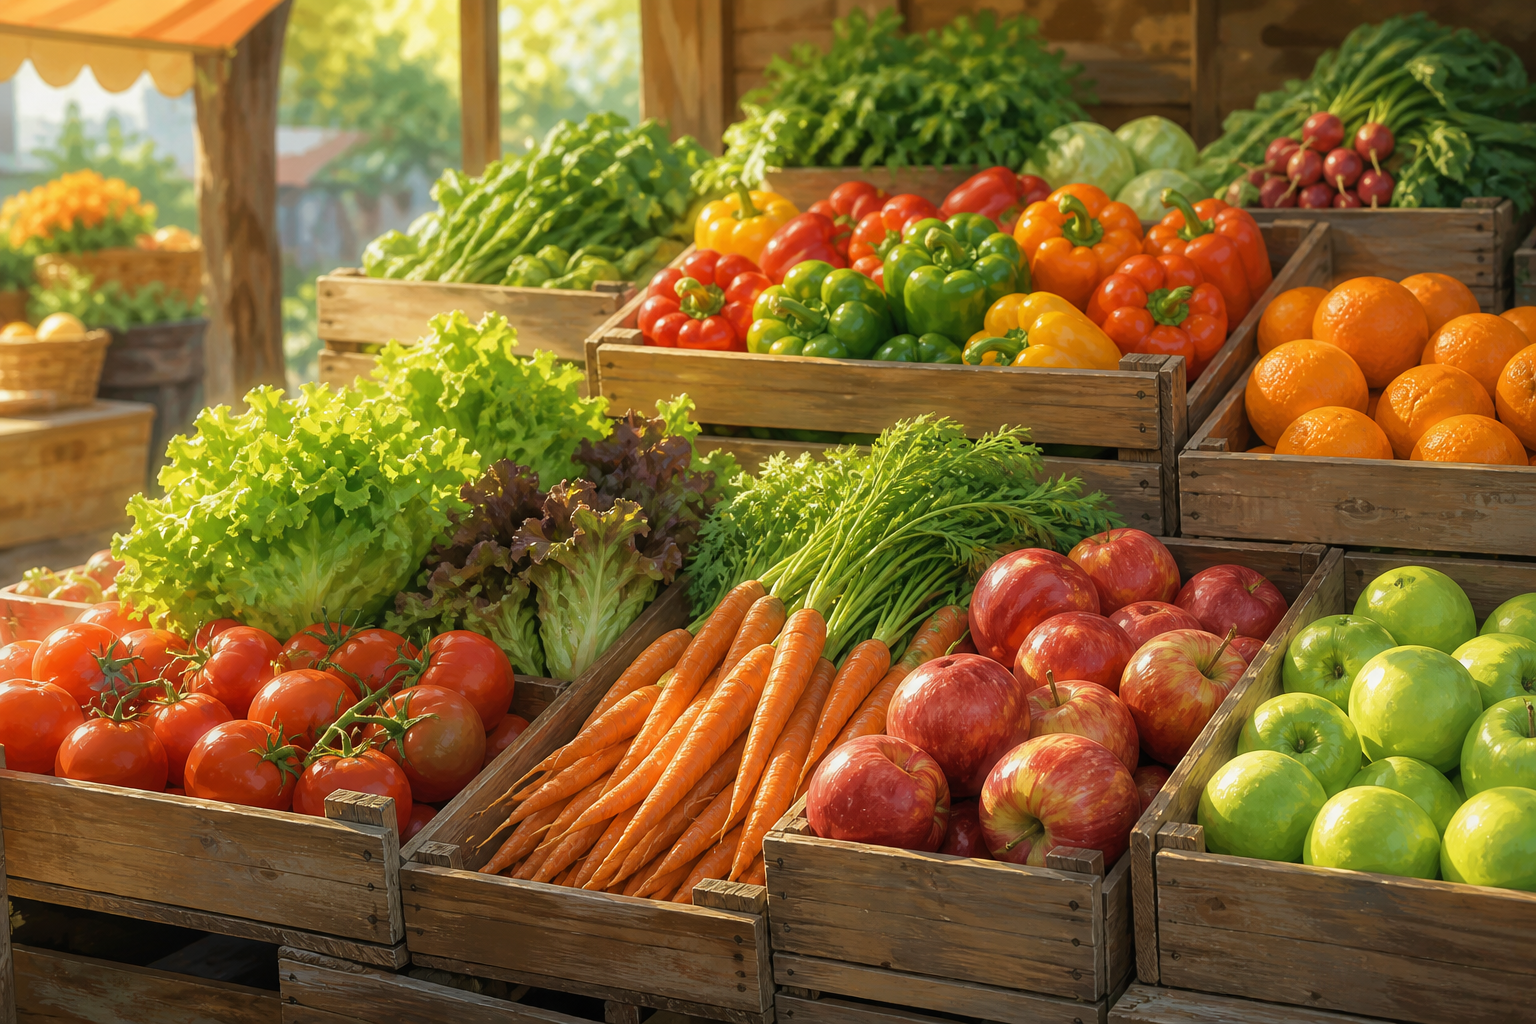
\includegraphics[width=0.62\linewidth]{images/book1/ai/g3-diet-market.png}

{\small De groep van de versheid op de markt: de hoek van het bord die
het vaakst vergeten wordt, hier zeker niet over het \omterm{def:g1:my-body:parts}{hoofd} te zien.}
\end{omfigure}

\begin{omfigure}
\begin{tikzpicture}
  % plate
  \draw[thick] (0,0) circle (2.8);
  % half: vegetables/fruit
  \draw[thick, fill=omMeth!14] (0,0) -- (0,2.8)
    arc[start angle=90, end angle=270, radius=2.8] -- cycle;
  % quarter: starchy
  \draw[thick, fill=omProp!14] (0,0) -- (0,-2.8)
    arc[start angle=270, end angle=340, radius=2.8] -- cycle;
  % quarter: builders
  \draw[thick, fill=omThm!12] (0,0) -- ({2.8*cos(340)},{2.8*sin(340)})
    arc[start angle=-20, end angle=90, radius=2.8] -- cycle;
  \node[font=\small, align=center] at (-1.4,0.2)
    {groente en\\ fruit\\ (de helft van het bord)};
  \node[font=\small, align=center] at (1.0,-1.45)
    {brood,\\ pasta, rijst};
  \node[font=\small, align=center] at (1.3,1.0)
    {vlees, vis,\\ ei of zuivel};
  % water glass
  \draw[thick] (4.0,-0.5) -- (4.1,1.0) -- (5.0,1.0) -- (5.1,-0.5)
    -- cycle;
  \fill[omDef!25] (4.04,-0.44) -- (4.12,0.75) -- (4.98,0.75)
    -- (5.06,-0.44) -- cycle;
  \node[font=\small, align=center] at (4.55,-1.0) {water om te drinken};
\end{tikzpicture}

{\small Een goed evenwichtig bord: de helft versheid, een kwart
langdurige \omterm{prop:g3:balanced-diet:jobs}{energie}, een kwart bouwers --- en water in het glas.}
\end{omfigure}

\begin{example}[Een lunch in evenwicht brengen]\label{ex:g3:balanced-diet:lunch}
Pasta met tomatensaus, een stuk vis, sperziebonen, een yoghurt, een
appel, water: elke groep aanwezig, lekkernijen afwezig --- een
evenwichtige lunch. Friet, een frisdrank en een reep chocola voeden
precies twee groepen (vetten en suiker) en slaan juist de groepen over
waar de bouwplaats op wachtte.
\end{example}

\begin{remark}[Geen verboden voedsel, alleen vergeten voedsel]\label{rem:g3:balanced-diet:balance}
Evenwicht wordt over dagen gemeten, niet over losse happen. Een punt
verjaardagstaart breekt geen enkele regel --- het probleem is nooit één
lekkernij, het zijn lekkernijen \emph{in plaats van} de groepen, dag na
dag. De praktische vraag bij elke maaltijd is niet ``is dit eten
slecht?'' maar ``welke groep ben ik vandaag vergeten?''
\end{remark}

\section{Voedsel afstemmen op de dag}

\begin{proposition}[Behoeften verschillen per dag en per persoon]\label{prop:g3:balanced-diet:needs}
Hoeveel \omterm{prop:g3:balanced-diet:jobs}{energie} een lichaam nodig heeft, hangt af van wie het is en wat
het doet: een groeiend kind heeft verhoudingsgewijs meer bouwmateriaal
nodig dan een volwassene; een dag sporten of winterkou verbrandt meer
\omterm{prop:g3:balanced-diet:jobs}{energie} dan een middag lezen. De honger groeit mee met wat het lichaam
uitgeeft.
\end{proposition}
\admitted

\begin{example}[Waarom het ontbijt telt]\label{ex:g3:balanced-diet:breakfast}
Tegen de ochtend heeft het lichaam de hele nacht doorgedraaid --- hart,
adem, warmte --- zonder ook maar één levering. Het ontbijt vult de
voorraad aan voor de lessen en het rennen van de ochtend. Sla het over,
en halverwege de ochtend komt de bouwplaats tekort: rommelende maag,
afdwalende aandacht, geen kracht bij het spelen.
\end{example}

\begin{method}[Het evenwicht van een dag nakijken]\label{met:g3:balanced-diet:check}
Loop aan het eind van de dag de lijst langs:
\begin{enumerate}
  \item groente of fruit bij elke maaltijd? (streven: ongeveer vijf
        porties op een dag)
  \item bij elke maaltijd iets zetmeelrijks voor langdurige \omterm{prop:g3:balanced-diet:jobs}{energie}?
  \item bouwers aanwezig --- zuivel een paar keer, en vlees, vis of
        eieren een- of tweemaal?
  \item water als drank van de dag?
  \item lekkernijen: een kleine hoeveelheid, geen hoofdrol?
\end{enumerate}
Welke groep er ook ontbreekt: nodig haar morgen uit.
\end{method}

\section{Oefeningen}

\begin{exercise}[$\star$]\label{exo:g3:balanced-diet:1}
Wat zijn de twee taken van voedsel? Geef één \omterm{def:g3:balanced-diet:families}{voedingsgroep} die vooral
elk van beide taken dient.
\end{exercise}

\begin{exercise}[$\star$]\label{exo:g3:balanced-diet:2}
Noem de \omterm{def:g3:balanced-diet:families}{voedingsgroepen}, en de enige drank die het lichaam nodig heeft.
\end{exercise}

\begin{exercise}[$\star$]\label{exo:g3:balanced-diet:3}
Deel deze boodschappen in groepen in: rijst, yoghurt, \omterm{def:g1:plants-around-us:parts}{wortels}, eieren,
boter, appels, brood.
\end{exercise}

\begin{exercise}[$\star$]\label{exo:g3:balanced-diet:4}
Waarom verbruikt het lichaam zelfs tijdens de \omterm{prop:g1:healthy-habits:needs}{slaap} \omterm{prop:g3:balanced-diet:jobs}{energie}? Noem twee
uitgaven van de nacht.
\end{exercise}

\begin{exercise}[$\star$]\label{exo:g3:balanced-diet:5}
Kijk de lunch ``pasta, vis, sperziebonen, yoghurt, appel, water'' na
tegen het evenwichtige bord uit de figuur: welk deel van het bord is
elk onderdeel?
\end{exercise}

\begin{exercise}[$\star$]\label{exo:g3:balanced-diet:6}
Waarom is het ontbijt bijzonder belangrijk? Wat gebeurt er halverwege
de ochtend zonder ontbijt?
\end{exercise}

\begin{exercise}[$\star$]\label{exo:g3:balanced-diet:7}
Wie heeft verhoudingsgewijs meer bouwmateriaal nodig: een kind of een
volwassene? Waarom?
\end{exercise}

\begin{exercise}[$\star$]\label{exo:g3:balanced-diet:8}
Probeer het: laat \cref{met:g3:balanced-diet:check} eerlijk over je
eigen dag lopen. Welke groep ben je vergeten --- en welke kwam er meer
voor dan haar deel?
\end{exercise}

\begin{exercise}[$\star\star$]\label{exo:g3:balanced-diet:9}
``Snoep is verboden!'' Is dat wat dit hoofdstuk zegt? Geef de
nauwkeuriger regel uit \cref{rem:g3:balanced-diet:balance}.
\end{exercise}

\begin{exercise}[$\star\star$]\label{exo:g3:balanced-diet:10}
Op wintersportvakantie heeft iedereen meer honger dan thuis. Leg het
uit met \cref{prop:g3:balanced-diet:needs} --- noem de twee extra
uitgaven die een koude, sportieve dag erbij geeft.
\end{exercise}
